\subsection{Fungi Interaction Model}
The \textit{Logistic model}~\cite{logisticmodel} can precisely analyze the growth phenomenon of animals, human and plants who naturally confront obstacles of survival attribute to the excess of the total population and the lack of food resources, so does microorganism, fungi. Therefore, it is suitable to use the \textbf{Logistic model} to study the interactions of different kinds of fungi.
\par
When a single fungal population lives, its number changes obey the \textbf{Single-group Logistic model}.
\begin{equation}
  \label{12eq}
  \frac{1}{N(t)}\frac{dN(t)}{dt} = r(1-\frac{N(t)}{N_{max}})
\end{equation}
where $N(t)$ represents current population size, and $r$ represents the growth rate of population.
When considering two fungal populations living together, due to competition for habitat and food, the interaction between them would hinder each other's growth and reproduction. Therefore, we introduce the \textbf{Relative Growth Blocking Index} (RGB) on the basis of Single-group Logistic model, and establish \textbf{Multi-groups Logistic Model}~\cite{multigroups} as follows.
\begin{equation}
  \begin{cases}
    \frac{1}{N_x(t)}\frac{dN_x(t)}{dt} = r_x(1-\frac{N_x(t)}{{N_x}_{max}} - RGB_x\frac{N_y(t)}{{N_y}_{max}}) \\ \\
    \frac{1}{N_y(t)}\frac{dN_y(t)}{dt} = r_y(1-\frac{N_y(t)}{{N_y}_{max}} - RGB_y\frac{N_x(t)}{{N_x}_{max}})
  \end{cases}
\end{equation}
where $N_x(t)$ and $N_y(t)$ represents the numbers of the two populations $x$ and $y$, $r_x$ and $r_y$ represents the inherent growth rate of populations, ${N_x}_{max}$ and ${N_y}_{max}$ are maximum capacities of populations, $RGB_x$ means for resources that support $x$, the consumption of $y$ is $RGB_x$ times the consumption of $x$ per unit quantity, and $RGB_y$ has the similar definition to $RGB_x$.
\par
Taking fungal species $F_A$ and $F_B$ proposed in the previous article as examples, analyze and predict the interaction between them. Calculate the values of parameters and list them as follows.
\begin{table}[H]
  \centering
  \caption{Values of parameters.}
  \label{valueofparameters}
  \begin{tabular*}{\hsize}{@{\extracolsep{\fill}}ccccc}
    \toprule
    \textbf{Parameter} & $RGB_A$ & $RGB_B$ & $r_A$ & $r_B$ \\
    \midrule
    \textbf{Value} & $0.39$ & $0.60$ & $1$ & $1$ \\
    \bottomrule
  \end{tabular*}
\end{table}
Draw the change curves of $N_A(t)$ and $N_B(t)$ as well as the phase trajectory of these two function variables as follows.
\par
\begin{figure}[H]
  \centering
  \subfigure[Curves of $N_A(t)$ and $N_B(t)$.]{
    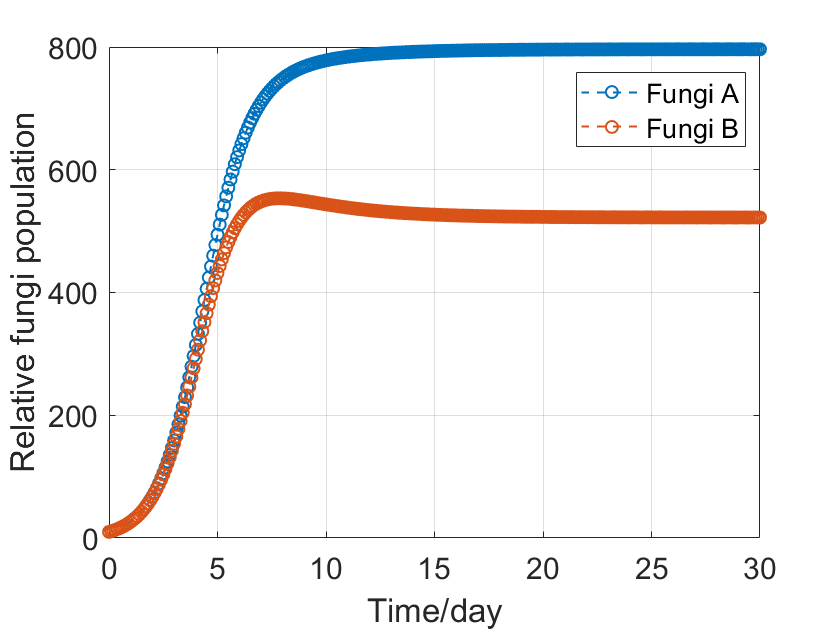
\includegraphics[width=0.48\textwidth]{figures/FA&FBN(t).png}
  }
  \subfigure[Phase trajectory of $N_A(t)$ and $N_B(t)$.]{
    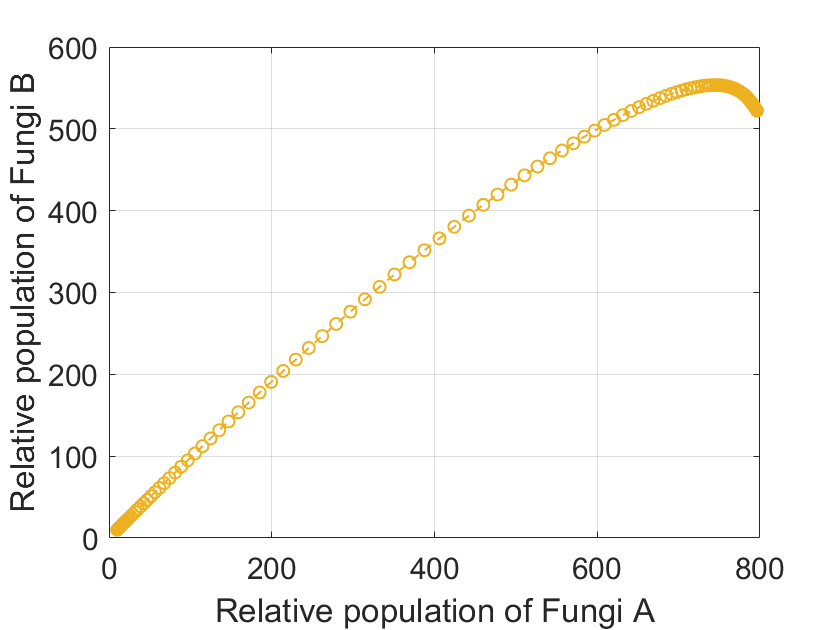
\includegraphics[width=0.48\textwidth]{figures/FA&FBline.png}
  }
  \caption{The interaction of $F_A\ \&\ F_B$.}
\end{figure}
\par
The dynamics of the interaction between Fungi A and Fungi B are characterized and described in the above figures. \textbf{In the short-term period} (about $1\sim 7$ days), $F_A$ and $F_B$ are in a period of rapid growth and reproduction, the curves of which maintain exponential growth. \textbf{In the long term} (after $8$ days), the growths of $F_A$ and $F_B$ would be both restricted by environmental resources. Meanwhile, because $F_A$ has a stronger ability to decompose, it has a stronger blocking effect on $F_B$. The final relative population numbers tend to $796$ and $522$ respectively and remain stable.
\par
In the same way, we calculate and analyze the interaction of Fungi C and Fungi E, and obtain the $N_C(t)$ and $N_E(t)$ function curves as well as the phase trajectory of the two function variables as follows.
\par
\begin{figure}[H]
  \centering
  \subfigure[Curves of $N_C(t)$ and $N_E(t)$.]{
    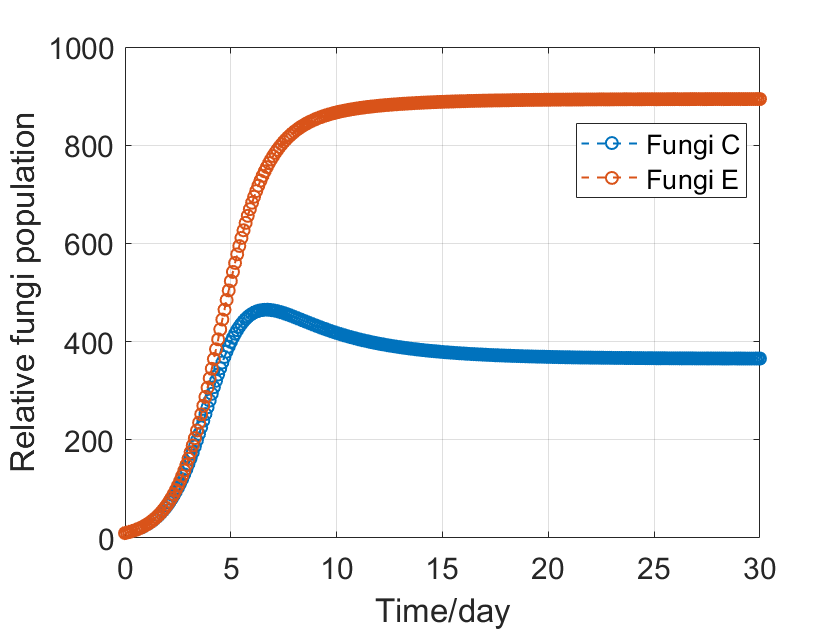
\includegraphics[width=0.48\textwidth]{figures/FC&FEN(t).png}
  }
  \subfigure[Phase trajectory of $N_C(t)$ and $N_E(t)$.]{
    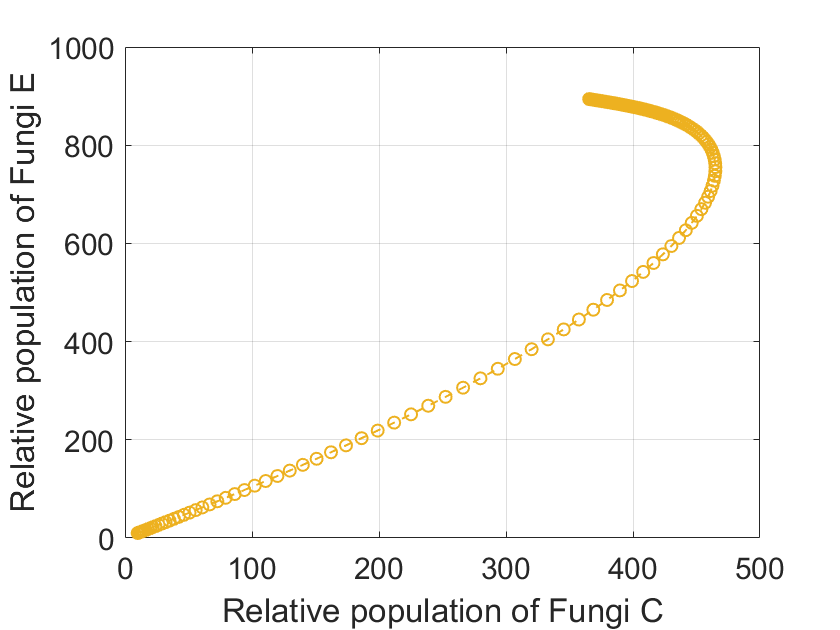
\includegraphics[width=0.48\textwidth]{figures/FC&FEline.png}
  }
  \caption{The interaction between $F_C\ \&\ F_E$.}
\end{figure}
\par
\textbf{In a short period of time} (about $1\sim 5$ days), the numbers of $F_C$ and $F_E$ grow exponentially. \textbf{From a long-term perspective} (after $6$ days), since the discrepancy of decomposition ability between $F_E$ and $F_C$ is greater than that between $F_A$ and $F_B$, the blocking effect of $F_E$ on $F_C$ is extremely obvious. The final relative populations numbers of $F_C$ and $F_E$ tend to $365$ and $894$ respectively and remain stable.